\documentclass[]{beamer}

\usepackage{lipsum}
\usepackage{pgfpages}
\usepackage{graphics}

\graphicspath{{img/}}

\mode<handout>{%
%	\setbeameroption{show notes}
}

\usetheme{AnnArbor}
\usecolortheme{beaver}

\AtBeginSection[]
{
	\begin{frame}
		\frametitle{Inhoudsopgave}
		\tableofcontents[currentsection]
	\end{frame}
}


\begin{document}
	\title[Actieherkenning met de Kinect sensor]{Live actieherkenning met de Kinect sensor in Python}
	\author[Bert De Saffel]{
				\begin{tabular}{rcr}
				prof. dr. ir. Peter Veelaert &\&& prof. dr. ir. Wilfried Philips \\
				ing. Sanne Roegiers &\&& ing. Dimitri van Cauwelaert
				\end{tabular}
	}
	
	\subtitle{Master of Science in de industriële wetenschappen: informatica \\ \vspace{0.2cm} Bert De Saffel}
	\date{13 februari 2019}
	\frame{\titlepage}
	
	\section{Context}
	
	\begin{frame}
	\frametitle{Context}
		\begin{itemize}
			\item<2- > Onderzoek naar menselijke actieherkenning
			\item<3- > Kinect Sensor 
			\begin{itemize}
				\item<3- > Genereert skelet via dieptebeelden
				\item<3- > Skelet wordt getransformeerd tot features
				\item<3- > Features worden gebruikt om pose of actie te classificeren
			\end{itemize}
		\end{itemize}
		\begin{figure}
			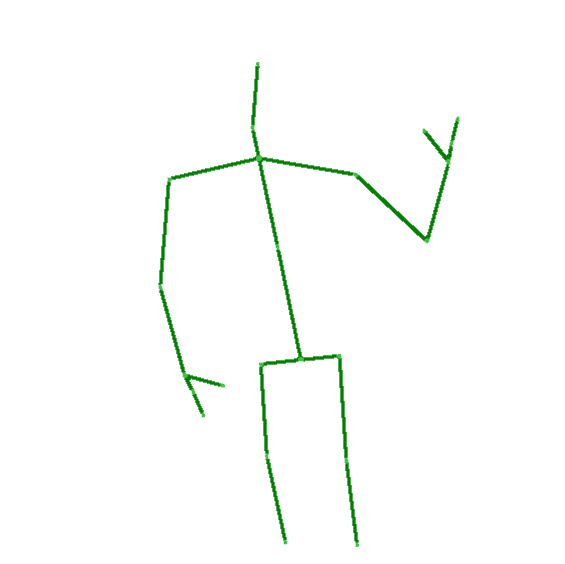
\includegraphics[width=0.4\textwidth]{skeleton}
		\end{figure}
	\end{frame}

	
	\section{Probleemstellingen}
	\subsection{Probleemstellingen}
	\begin{frame}
	\frametitle{Probleemstellingen}

		\begin{enumerate}
			\item<1- > Invariant zijn van de features, onafhankelijk van o.a.:
				\begin{itemize}
				\item verschillen in lichaamsbouw
				\item actie-uitvoering
				\item camerahoek
				\end{itemize}
			\item<2- > Python implementatie voor de Kinect sensor
				\begin{itemize}
				\item Live mapping van de verschillende sensoren
				\item Beelden opslaan in toegankelijk videoformaat
				\end{itemize}
			
		\end{enumerate}
		\begin{figure}
			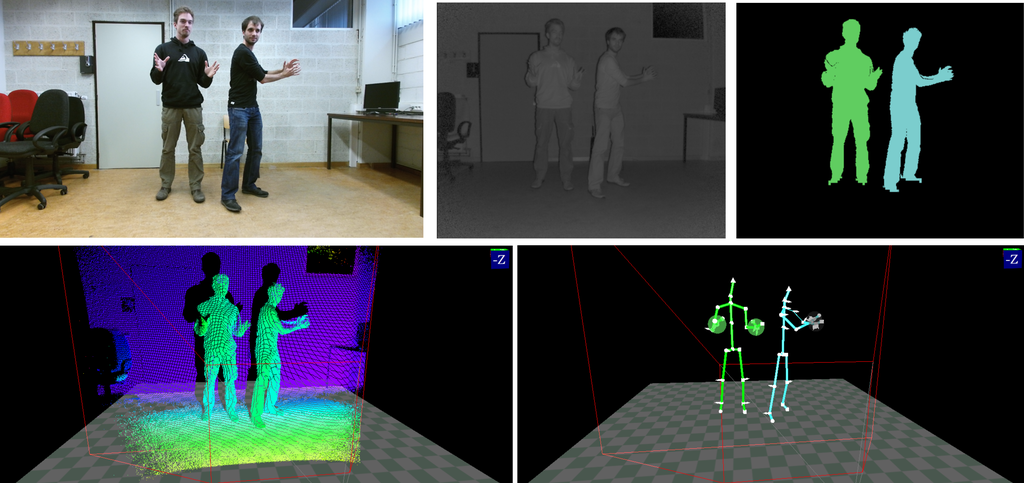
\includegraphics[width=0.6\textwidth]{sensoren}
		\end{figure}

	\end{frame}
	\note[itemize]{
		\item Live actieherkenning: eenvoudige acties, invariant voor verschillen in lichaamsbouw, actie-uitvoering en camerahoek.
		\item Python implementatie: live mapping van beelden + opslaan in toegankelijk videoformaat

	}
	
	\subsection{Gewenst eindresultaat}	
	\begin{frame}
	\frametitle{Gewenst eindresultaat}
		\begin{itemize}
			\item<1- > Wat? 
				\begin{itemize}
				\item<1- > Prototype
				\item<1- > Snelle, eenvoudige actieherkenning in robuuste omgeving
				\item<1- > Beelden beschikbaar in toegankelijk videoformaat
				\end{itemize}
			\item<2- > Waarom nuttig?
				\begin{itemize}
				\item<2- > Uitbreidmogelijkheden: interactie mens-robot, analyseren fitnessoefeningen, ...
				\item<2- > Demonstratie op opendeurdag
				\end{itemize}
			
		\end{itemize}
	\end{frame}
	\note[itemize]{
		\item Wat? Prototype $\rightarrow$ snelle eenvoudige actieherkenning in robuuste omgeving (bv opendeurdag: veel mensen) $\rightarrow$ tonen op scherm $\rightarrow$ informatie (de beelden) beschikbaar in databank $\rightarrow$ toegankelijk videoformaat (vs .xef in Kinect Studio: neemt te veel schijfruimte in)
		\item Waarom nuttig? 
			Uitbreidmogelijkheden: interactie mens-robot, analyseren fitnessoefeningen, ...
			Demonstratie op opendeurdag
	}

	\section{Plan van aanpak}
	\subsection{Literatuurstudie}
	\begin{frame}
	\frametitle{Literatuurstudie}
		Planning: 04/feb - 17/feb
		\begin{figure}
		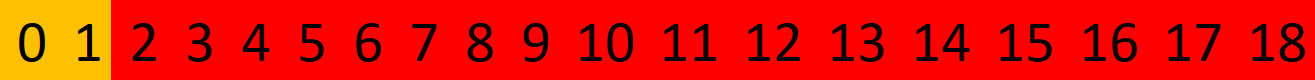
\includegraphics[width=\textwidth]{literatuur}
		\end{figure}
		\begin{itemize}
			\item<1- > Mogelijkheden en limitaties van de kinect sensor
			\item<1- > Bestaande actieherkenningsalgoritmen bestuderen
			\item<1- > Bestuderen bestaande implementaties Kinect code
			\item<1- > Klaarzetten werkomgeving
		\end{itemize}
	\end{frame}
	\note[itemize]{
		\item Derde punt: Eerder voor mezelf als de basis van de python wrapper, geen stuk in de thesis zelf
	}

	\subsection{Python wrapper}
	\begin{frame}
	\frametitle{Python wrapper}
		Planning: 18/feb - 17/mrt
		\begin{figure}
		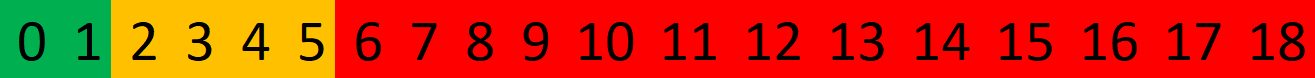
\includegraphics[width=\textwidth]{wrapper}
		\end{figure}
		\begin{itemize}
			\item<1- > Kinect sensor aanspreken vanuit Python
			\item<1- > Twee hoofdfunctionaliteiten:
			\begin{itemize}
				\item<1- > Live mapping van de Kinect sensoren
				\item<1- > Opslaan beelden in toegankelijk videoformaat
			\end{itemize}
			\item<1- > Testen
		\end{itemize}
	\end{frame}
	\note[itemize]{
		\item Gepland voor week 2 - 5
		
		\item sensoren: kleurenbeelden, dieptebeelden, infraroodbeelden, body index beelden en skeletdata
	}

	\subsection{Actieherkenning met machine learning}
		\begin{frame}
		\frametitle{Actieherkenning met machine learning}
		Planning: 18/mrt - 26/mei
		\begin{figure}
		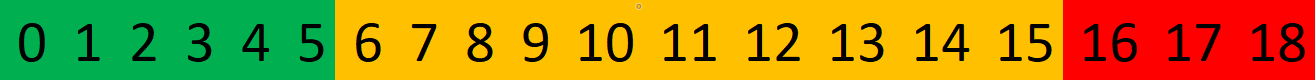
\includegraphics[width=\textwidth]{actieherkenning}
		\end{figure}
		\begin{itemize}
			\item<1- > Toepassen/uitbreiden van bestaande actieherkenningalgoritmen
			\begin{itemize}
				\item Op één enkel persoon
				\item Op meerdere personen
			\end{itemize}
			\item<2- > Training data: bestaande datasets
		\end{itemize}
	\end{frame}
	\note[itemize]{
		\item Gepland voor week 6-14 ; week 15 en 16 zijn buffer (week 18 indienen)
	
		\item Gebruik maken van gekende actieherkenningalgoritmen om probleemstelling aan te pakken.
	
		\item bestaande datasets: bv Human Motion DataBase (HMDB51), UT Kinect 
		
		\item alternatief: zelf beelden maken
	}
	
	\begin{frame}
	\frametitle{Buffer}
	Overige weken: 27/mei - 10/jun
	\begin{figure}
		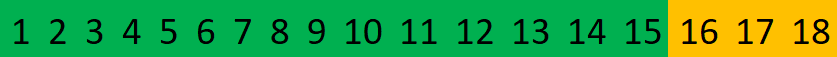
\includegraphics[width=\textwidth]{buffer}
	\end{figure}
	\begin{itemize}
	\item Bufferperiode
	\item Afwerken scriptie
	\end{itemize}
	\end{frame}
	
	\begin{frame}
		\begin{center}
			\Huge Vragen, opmerkingen, ...?
		\end{center}
	\end{frame}
\end{document}